\documentclass[12pt]{article}
\usepackage[margin=1in]{geometry}
\usepackage[english,russian]{babel}
\usepackage{amsmath,amsthm,amssymb,color,latexsym}
\usepackage{geometry}        
\geometry{letterpaper}    
\usepackage{graphicx}

\newtheorem{problem}{Задача}

\newenvironment{solution}[1][\it{Решение}]{\textbf{#1. } }{$\square$}


\begin{document}
	\noindent Наблюдательная астрофизика\hfill Экзамен\\
	Збродов Владислав 22.С03
	
	\hrulefill
	\section{Блок. Базовые понятия.}
	\subsection{Основные задачи астрофизики и объекты исследований, наблюдательная астрофизика.}
	\textbf{Астрофизика} – раздел астрономии, изучающий физические
	свойства космических объектов и происходящие в них процессы на
	основе общих физических законов.\\
	\\
	\textbf{Что изучает астрофизика:}
	\begin{itemize}
	\item	Строение и эволюция звёзд;
	\item Экзопланеты;
	\item Межзвёздная среда;
	\item Галактика;
	\item Эволюция галактик;
	\item Космология.
	\end{itemize}
	
		\textbf{Основные задачи астрофизики:}
	\begin{itemize}
		\item	Изучение структуры и эволюции звезд:
			\begin{enumerate}
				\item Понимание процессов, происходящих внутри звезд, их жизненного цикла, от рождения до смерти.
				\item Исследование звездных классификаций, спектральных типов и их физических свойств.
			\end{enumerate}
		
		
		\item Исследование галактик:
			\begin{enumerate}
				\item 	Изучение структуры, динамики и эволюции галактик.
				\item 	Исследование активных галактических ядер и квазаров.
				\item 	Понимание процессов звездообразования и взаимодействия галактик.
			\end{enumerate}
		\item Космология:
			\begin{enumerate}
				\item 	Изучение происхождения, структуры и эволюции Вселенной.
				\item 	Исследование темной материи и темной энергии.
				
				\item 	Понимание космического микроволнового фона.
			\end{enumerate}
		\item Планетарные системы:
			\begin{enumerate}
				\item 	Изучение состава, структуры и динамики межзвездного газа и пыли.
				\item 	Исследование молекулярных облаков и процессов звездообразования.
			\end{enumerate}
		\item Высокоэнергетические явления:
		\begin{enumerate}
			\item 	Изучение сверхновых, гамма-всплесков, нейтронных звезд и черных дыр.
			\item Исследование космических лучей и высокоэнергетических частиц.
		\end{enumerate}
	\end{itemize}
	Наблюдательная астрофизика играет ключевую роль в понимании Вселенной, предоставляя данные, которые позволяют астрофизикам тестировать и уточнять теоретические модели.
	
	\subsection{Используемые инструменты, методы и источники информации об исследуемых объектах.} 
	\textbf{Наблюдательная астрофизика} использует широкий спектр инструментов, методов и источников информации для изучения различных астрономических объектов.
	\textbf{Инструменты наблюдательной астрофизики:}
	\begin{itemize}
		\item \textbf{Оптические телескопы:}
				\begin{enumerate}
				\item 	\textbf{Наземные телескопы}: Большие оптические телескопы, такие как Keck, VLT (Very Large Telescope), и Subaru, используются для наблюдений в видимом и ближнем инфракрасном диапазонах.
				\item \textbf{Космические телескопы}: Хаббл (Hubble Space Telescope) и Джеймс Уэбб (James Webb Space Telescope) предоставляют высококачественные изображения и спектры без атмосферных помех.
			\end{enumerate}
		\item\textbf{Радиотелескопы}:	
				\begin{enumerate}
				\item 	\textbf{Наземные радиотелескопы}: ALMA (Atacama Large Millimeter/submillimeter Array), VLA (Very Large Array), и LOFAR (Low-Frequency Array) используются для наблюдений в радиодиапазоне.
				\item \textbf{Космические радиотелескопы}: Радиотелескопы на орбите, такие как Spektr-R, позволяют избежать атмосферных помех.
			\end{enumerate}
			
			\item\textbf{Инфракрасные телескопы}:	
		\begin{enumerate}
			\item 	\textbf{Наземные инфракрасные телескопы}: IRTF (Infrared Telescope Facility) и UKIRT (United Kingdom Infrared Telescope).
			\item \textbf{Космические инфракрасные телескопы}: Spitzer Space Telescope и Herschel Space Observatory.
		\end{enumerate}	
		
		
			\item\textbf{Ультрафиолетовые телескопы}:	
				\begin{enumerate}
				\item 	\textbf{Космические ультрафиолетовые телескопы}: GALEX (Galaxy Evolution Explorer) и Swift.
			\end{enumerate}	
			
		\item\textbf{Рентгеновские телескопы}:	
		\begin{enumerate}
			\item 	\textbf{Космические рентгеновские телескопы}:Chandra X-ray Observatory и XMM-Newton.
		\end{enumerate}	
		
		\item\textbf{Гамма-телескопы}:	
		\begin{enumerate}
			\item 	\textbf{Космические гамма-телескопы}: Fermi Gamma-ray Space Telescope.
				\item 	\textbf{Наземные гамма-телескопы}: Cherenkov Telescope Array (CTA) и HESS (High Energy Stereoscopic System).
		\end{enumerate}		
	\end{itemize} 
	
		\textbf{Методы наблюдательной астрофизики:}
	\begin{itemize}
		\item \textbf{Фотометрия:}
		\begin{enumerate}
			\item Измерение яркости небесных объектов в различных диапазонах спектра.
			\item Используется для определения светимости, температуры и расстояния до объектов.
		\end{enumerate}
		\item\textbf{Спектроскопия}:	
		\begin{enumerate}
			\item Анализ спектров небесных объектов для определения их состава, температуры, скорости и других физических параметров.
			\item Используется для изучения химического состава звезд, галактик и межзвездной среды.
		\end{enumerate}
		
		\item\textbf{Интерферометрия}:	
		\begin{enumerate}
			\item Использование нескольких телескопов для создания виртуального телескопа с высоким разрешением.
			\item Применяется в радиоастрономии (VLBI) и оптической астрономии (VLTI).
		\end{enumerate}	
		
		
		\item\textbf{Поляриметрия}:	
		\begin{enumerate}
			\item 	Измерение поляризации света от небесных объектов.
			\item Используется для изучения магнитных полей и структуры межзвездной среды.
		\end{enumerate}
	\end{itemize}
	Приёмники излучения используются для обнаружения и анализа ЭМ излучения от объектов. В зависимости от диапазона спектра, применяются различные типы приёмников.\\
	\textbf{Источники информации об исследуемых объектах:}
	\begin{itemize}
		\item Электромагнитное излучение;
		\item Нейтрино;
		\item Гравитационные волны;
		\item Космические лучи.
	\end{itemize}
	
	
	
	\subsection{Электромагнитное излучение, основные характеристики и единицы измерений.}
	
	Основным источником информации о небесных телах остаётся ЭМ излучение.
	Спектральный состав характеризуется длиной волны
	излучения $\lambda$ или частотой $\nu$.
	
	\begin{center}
		\begin{tabular}{||c c c||} 
			\hline
			Диапазон & Энергия($h\nu$) &Температура ($h\nu/k$) \\ [0.5ex] 
			\hline\hline
			Гамма лучи & $10^5$ эВ& $10^9$ К  \\ 
			\hline
			X & $10^3$ эВ& $10^7$ К  \\
			\hline
			УФ & $10$ эВ& $10^5$ К  \\
			\hline
			Видимый & $1$ эВ& $10^4$ К  \\
			\hline
			ИК & $0.1$ эВ& $10^3$ К   \\
			\hline
			Микроволновый & $10^{-3}$ эВ& $10$ К   \\
			\hline
			Радио & $10^{-6}$ эВ& $0.001$ К   \\
			\hline
		\end{tabular}
	\end{center}
	\textbf{dQ} -- энергия от источника.
	\textbf{Поток излучения - энергия, протекающая через площадку $dA$ за время $dt$.}
	$$F = \frac{dQ}{dt}$$ 	Измеряется в эрг/с или других единицах мощности, например в
	ваттах.
\begin{figure}[h]
	\centering
	\includegraphics[width=0.3\linewidth]{"111"}
\end{figure}\\
	Освещенность или плотность потока -- пото с единичной площадки $dS$:
	$$E = \frac{dF}{dS}$$ Измеряется в эрг/с/см$^2$\\
	\textbf{Интенсивность точечного источника}
	$$I = \frac{dF}{d\Omega}$$
	$$d\Omega = \frac{dS}{r^2}$$
	Характеризует излучательные свойства источника, и не зависит от того, на каком расстоянии от него поместить элементарную площадку.	\\
	\textbf{Поверхностная яркость протяженного источника:}
	$$B = \frac{I}{\sigma}$$
	$\sigma$ -- проекция площадки на плоскость, перпендикулярную направлению распространения света, измеряется в эрг/с/стерад/см$^2$\\
	Удельная плотность потока измеряется в ватт/м$^2$/Гц, Янский (1 Ян $= 10^{-26}$ ватт/м$^2$/Гц)\\
	Переход от $\nu$ к $\lambda$:
	$$\lambda E_{\lambda}= \nu E_{\nu}$$
	\textbf{Пример}:
	Удельная освещенность на $10^8$ Гц ($\lambda = 300$ см)
	составляет $E_{\nu}	= 17\cdot10^{-23}$ вт/м$^2$/Гц.
	\subsection{Земная атмосфера, её влияние, условия наблюдений, внеатмосферные источники искажений.}
	Земная атмосфера оказывает значительное влияние на наблюдения в астрономии, как в оптическом, так и в других диапазонах электромагнитного спектра. \\
	\textbf{Земная атмосфера:}
	\begin{itemize}
		\item Поглощение и рассеяние света:
			\begin{enumerate}
				\item \textbf{Поглощение}: Молекулы и аэрозоли в атмосфере поглощают свет определенных длин волн, что приводит к ослаблению сигнала от астрономических объектов. Например, озон в атмосфере поглощает ультрафиолетовое излучение, а водяной пар поглощает инфракрасное излучение.
				\item \textbf{Рассеяние}: Рассеяние света на молекулах и частицах в атмосфере (так называемое рассеяние Рэлея) приводит к уменьшению яркости объектов и ухудшению контраста изображений.
			\end{enumerate}
			\begin{figure}[h]
				\centering
				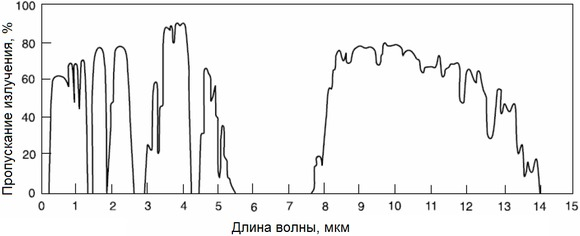
\includegraphics[width=0.7\linewidth]{atmosphere}
			\end{figure}
			Рассеяние света: на молекулах воздуха, коэффициент рассеяния пропорционален $\sim \lambda^{-4}$,
		на аэрозоле коэффициент пропорционален $ \sim \lambda^{-\alpha} $, где $ \alpha \approx 0.8$;
		\item \textbf{Атмосферная помутненность}: Турбулентность в атмосфере вызывает колебания плотности воздуха, что приводит к искажению волнового фронта света, проходящего через атмосферу. Это явление называется атмосферной помутненностью и ограничивает угловое разрешение наземных телескопов.
		
		\item \textbf{Атмосферная дисперсия}: Различные длины волн света преломляются в атмосфере по-разному, что приводит к хроматической аберрации и искажению изображений.
	\end{itemize}

	\textbf{Условия наблюдений:}
	\begin{itemize}
		\item \textbf{Высокогорные обсерватории}: Расположение обсерваторий на высоких горах (например, Мауна-Кеа на Гавайях) снижает влияние атмосферы, так как количество атмосферы над телескопом уменьшается.
		\item \textbf{Сухие и стабильные климатические условия}: Обсерватории часто строятся в пустынных или полупустынных районах с низкой влажностью и стабильной погодой, что снижает влияние водяного пара и атмосферной турбулентности.
	\end{itemize}
	
	\textbf{Внеатмосферные источники искажений:}
	\begin{itemize}
		\item \textbf{Космические лучи}: Высокоэнергетические частицы, попадающие в атмосферу Земли, могут создавать фоновый шум и искажения в детекторах.
		\item \textbf{Солнечный свет}: Рассеянный солнечный свет может создавать фоновый шум, особенно при наблюдениях в дневное время или в сумеречное время.
		\item \textbf{Ионосфера}: Ионосфера Земли может искажать радиосигналы, особенно на низких частотах.
	\end{itemize}
	
	\textbf{Способы избежать влияния атмосферы:}
	\begin{enumerate}
		\item \textbf{Космические телескопы}: Размещение телескопов на орбите Земли позволяет полностью избежать влияния атмосферы. Примеры космических телескопов включают Хаббл (Hubble Space Telescope) для оптических и ультрафиолетовых наблюдений, Чандра (Chandra X-ray Observatory) для рентгеновских наблюдений и Спитцер (Spitzer Space Telescope) для инфракрасных наблюдений.
		\item \textbf{Баллонные и высотные наблюдения}: Использование воздушных шаров и высотных самолетов позволяет поднять телескопы на большие высоты, где влияние атмосферы минимально. Примеры включают SOFIA (Stratospheric Observatory for Infrared Astronomy), который размещен на борту самолета.
	\end{enumerate}
	
	\section{Блок. Оптические телескопы и инструменты.}
	\subsection{Функции телескопа, его основные характеристики и ограничения.}
	Телескоп является основным инструментом в наблюдательной астрофизике, позволяя астрономам собирать свет от далеких объектов и анализировать его для получения информации о Вселенной.\\
		\textbf{Задачи телескопа}: Прием и анализ излучения
		осуществляется с помощью
		телескопа.
	\begin{enumerate}
		\item Собрать и направить на приемник излучения как
		можно большее количество световой энергии;
		\item Отделить положения изображений источников (или
		отдельных деталей) друг от друга;
		\item Выделить сигнал от отдельного источника среди
		естественного шума.
	\end{enumerate}
	\textbf{Функции телескопа}:
	\begin{enumerate}
		\item Увеличение угла зрения (увеличение видимых размеров объекта и разрешения близко расположенных объектов) – по существу приближение объекта.
		\item Увеличение плотности потока (и, тем самым, проницающей силы).
		\item Направление излучения от объекта на приёмник.
	\end{enumerate}
	\textbf{Характеристики телескопа}:
	\begin{enumerate}
		\item Угловое увеличение (Увеличение одиночной линзы).\\
		Равнозрачковое увеличение: $g = D/\delta$, $D$ -- диаметр зеркала, $\delta$ — диаметр зрачка.		
		\item Масштаб изображения -- какой линейный размер в
		фокальной плоскости будет соответствовать угловому
		расстоянию на небе. $L = F \tg{\alpha}$, $\tg{\alpha} \approx \alpha$, $L \approx F \alpha''/ 206265''$
		\item Поле зрения -- угловой размер области неба,
		которую телескоп может качественно отобразить на
		приёмнике излучения.
			\begin{itemize}
				\item Зеркально -- линзовые телескопы системы
				Шмидта и Максутова -- максимальное поле
				зрения $5^{\circ} - 6^{\circ}$
				\item Рефлекторы -- $1^{\circ}$
				\item Визуальные наблюдения -- ограничения окуляра.
				\item Относительное отверстие телескопа -- $A = D/F$ (светосила)
				\item Разрешение -- способность различать
				мелкие детали. (человеческий глаз $\sim1'$)
				\item Теоретическое разрешение $\alpha[rad] = 1.22 \lambda/D$\\
				$a = F\alpha = 1.22 \lambda F/D$ -- линейный радиус кольца.
				\item Разрешающая сила телескопа -- 
				При $\Delta$ между двумя звёздами меньше $2\alpha$
				частичное наложение дифракционных дисков;
				Предел разрешающей силы телескопа:
				$\Delta'' = 0.85 \alpha$
				\item Проницающая сила – способность телескопа
				регистрировать слабые объекты. (Для глаза – $5^{m} - 6^{m}$)
				$$m = 2 + 5\lg D [mm]$$
			\end{itemize}
			
	\end{enumerate}
	
	
	\subsection{Основные типы телескопов, классические оптические схемы, аберрации оптических систем, потери и ограничения.}
	\subsection{Конструкция телескопов и типы монтировок. Тонкие и сегментированные зеркала. Активная и адаптивная оптика.}
	\subsection{Солнечные телескопы. Целостат, внезатменный коронограф и космические солнечные телескопы.}
	\subsection{Особенности ИК-телескопов. Телескопы для далекого ультрафиолета и рентгеновского излучения, космические ИК/УФ/X телескопы.}
	\subsection{Оптические интерферометры. Интерферометр Фабри - Перо.}
	\subsection{Фотометры, поляриметры, светофильтры.}
	\subsection{Спектрографы. Оптическая схема, призмы и дифракционные решётки. Мультизрачковый и мультиобъектный спектрографы.}
	\section{Блок. Приёмники излучения.}
\subsection{Основные типы и основные характеристики и ограничения приемников излучения, типы шумов.}
\subsection{Приемники излучения, работающие на внешнем фотоэффекте.}
\subsection{Одноканальные приемники на внутреннем фотоэффекте. Тепловые приемники.}
\subsection{ПЗС и ПЗС-матрицы.}
\subsection{Приёмники УФ и рентгеновского диапазонов, способы определения направления излучения.}
\subsection{Приёмники и способы регистрации гамма-квантов, способы определения направления излучения}
\subsection{Регистрация космических лучей.}
\subsection{Нейтринные детекторы, способы регистрации гравитационных волн.}
	
\end{document}
